\documentclass{article}
\usepackage{graphicx} 
\usepackage{adjustbox}
\usepackage{float}
\usepackage{listings}
\usepackage{xcolor}
\usepackage{amsmath}
\usepackage{hyperref}
\hypersetup{
    colorlinks=true,
    urlcolor=blue,
    linkcolor=black,
    citecolor=black
}
\usepackage[section]{placeins}


\definecolor{codebg}{rgb}{0.97,0.97,0.97}
\lstset{
  backgroundcolor=\color{codebg},
  basicstyle=\ttfamily\small,
  breaklines=true,
  frame=single,
  columns=fullflexible,
  keepspaces=true,
  captionpos=b,
  language=JavaScript,
  showstringspaces=false
}

\title{whitepaper}
\author{Yash Singh}
\date{July 2025}

\usepackage[section]{placeins}

\title{Tychi Protocol – Technical Whitepaper}
\author{Yash Singh \\ Tychi Labs (part of Tychi Ltd) \\ yash@tychiwallet.com}
\date{Version: v0.5.0 (Testnet) \\ July 2025}

\begin{document}
\maketitle

\textbf{\footnotesize Legal Disclaimer}\scriptsize
~~Nothing in this Whitepaper constitutes an offer to sell, or the solicitation of an offer to buy, any tokens, products, or services. Tychi Labs is publishing this Whitepaper solely for informational purposes and to solicit community feedback and technical comments.

If and when Tychi Labs, under the entity UGF, decides to offer any tokens (or enter into any form of agreement such as a Simple Agreement for Future Tokens – SAFT), it will do so through formal offering documents, which will include risk disclosures, legal terms, and a revised version of this Whitepaper. Such offerings, if conducted in jurisdictions like the United States, will likely be limited to accredited investors in compliance with applicable laws.

This document does not constitute legal, financial, or investment advice, and should not be treated as such. No representations or warranties are made as to the accuracy or completeness of any information contained herein, nor should any part of this Whitepaper be interpreted as a guarantee of future performance, token utility, or ecosystem development.

Plans and features described in this document are subject to change at the sole discretion of Tychi Labs. The success and adoption of the Tychi Protocol will depend on numerous external factors, including but not limited to regulatory developments, market conditions, and technological advancements.

Readers are strongly advised to consult their own legal, financial, and tax advisors before making any decisions related to the Tychi ecosystem.

\section*{Abstract}

The Universal Gas Forwarder (UGF) is a cross-chain transaction execution protocol developed by Tychi Labs that enables users to prepay gas on one blockchain and execute transactions on another. Designed to simplify and unify cross-chain user experiences, UGF abstracts away the complexity of multi-network gas requirements by introducing a seamless transaction relay layer powered by smart wallets, fuel prepayment contracts, and multi-relayer validation. Currently live on testnet, UGF supports EVM chains, Solana, and Sui, offering a gas-abstracted gateway to truly interoperable blockchain applications.


\section*{Why Cross-Chain Isn’t Seamless}

Let’s say you’re a user who primarily operates on BNB Chain — you trade there, hold assets, and it's where most of your gas balance sits. But over time, you start interacting with other ecosystems. A client pays you on Solana. Airdrops or DeFi opportunities appear on Ethereum or Sui. You now have assets on multiple chains — but they’re stuck.

To actually use your tokens, two major problems emerge:

\begin{itemize}
  \item \textbf{You need to buy native gas on each chain — just to make a transaction.}  
  Even if you already hold tokens on Solana or Ethereum, you can’t move or trade them unless you first acquire SOL or ETH separately, often through a centralized exchange or bridge.
  
  \item \textbf{Your liquidity is fragmented across chains, and accessing it requires bridging or wrapping.}  
  Want to use an opportunity on one chain? You’re forced to bridge your tokens from another chain — an extra step that is slow, costly, and error-prone.
\end{itemize}

These frictions break the promise of a seamless, interoperable crypto ecosystem and make cross-chain participation needlessly complicated.



\section*{Introducing Universal Gas Framework}

The Universal Gas Framework (UGF) is the core infrastructure layer behind Tychi Wallet’s cross-chain capabilities. It is designed to solve one of the most persistent UX bottlenecks in blockchain: fragmented gas fees across networks.

With UGF, users no longer need to acquire and manage native gas tokens on every chain they interact with. Instead, they hold BNB on a single low-cost network — opBNB — and use it to prepay for transactions across multiple chains. Whether the user wants to execute on Ethereum, BNB Chain, Solana (for SPL token transfers), or Sui (for sponsored Move contract calls), UGF handles the complexity of gas forwarding and execution beneath the surface.

\textbf{Version v0.1} of UGF supports:
\begin{itemize}
  \item EVM chains (e.g., Ethereum, BNB Testnet, Sepolia)
  \item Solana (SPL token transfers)
  \item Sui
\end{itemize}

In upcoming releases, we will introduce a developer SDK to allow seamless UGF integration into third-party wallets, dApps, and service layers — further abstracting away the need for users to think about gas management at all.

\textbf{UGF is the invisible layer that lets users pay once and execute anywhere — bringing true interoperability to life.}



\section*{Design Philosophy: Why We Built UGF This Way}

The Universal Gas Framework (UGF) was designed with a single premise in mind: users shouldn’t have to think about gas — especially not across chains. In today’s fragmented Web3 ecosystem, every blockchain demands its own native gas token. This requirement disrupts user experience at a fundamental level. Sending tokens on Ethereum requires ETH. Claiming an airdrop on Solana requires SOL. Even simple DeFi actions often involve manual gas top-ups through CEX withdrawals or cross-chain bridges. UGF was built to eliminate this friction entirely.

Our goal was to make cross-chain interaction feel seamless — not like a series of disconnected steps. We envisioned a system where users could hold gas on a single chain, pay once, and execute transactions on any supported network. To accomplish this, we introduced a number of foundational components and principles.

On EVM-based chains, UGF deploys per-user smart wallets that support gasless transactions, flexible signature validation, and nonce management. For Solana and Sui — which currently operate with EOAs — the v0.5.0 release supports direct signed SPL and Move instructions, with future plans to introduce smart wallet abstraction there as well. To securely manage gas prepayment, FuelStation contracts are deployed on the designated payment chain (opBNB in this release). These contracts handle quote validation, replay protection, and serve as the trust anchor for the entire system.

Rather than using traditional bridging mechanisms, UGF leverages a decentralized network of relayers that independently validate and co-sign each transaction. This multi-relayer consensus model enhances both security and execution speed, enabling near real-time cross-chain interactions. The system is designed to be chain-agnostic from the ground up. While the initial release supports EVM chains, Solana (SPL transfers), and Sui, the architecture is modular enough to onboard chains like Aptos, XRP, and even Bitcoin in later phases.

UGF is also being built with developers in mind. With the upcoming v1.5 release, we will introduce an SDK and API suite, making it easy for wallets, dApps, and platforms to integrate gas abstraction into their own user flows. Looking ahead, UGF may evolve into a dedicated execution layer of its own — potentially launching our own Blockchain for protocol-level coordination and TychiScan as a cross-chain transaction explorer.

With UGF v0.5.0, we are laying the foundation for a unified, gas-abstracted user experience — one where users can pay once, act anywhere, and never be blocked by fragmented infrastructure again.


\section*{Why opBNB and BNB?}

BNB is one of the most widely held and liquid assets in the crypto ecosystem. It’s accessible across major exchanges, supported by all major wallets, and deeply integrated into DeFi platforms — making it an ideal choice for gas payments.

To enable fast and cost-efficient execution, we chose \textbf{opBNB} as the gas payment network. Built as an Optimism-based Layer 2 secured by BNB Chain, \textbf{opBNB functions as an omnichain settlement layer} with extremely low fees, high throughput, and full EVM compatibility — perfect for powering real-time gas abstraction at scale.

Users only need to hold BNB on opBNB to interact with UGF. If needed, they can easily bridge BNB using the official \href{https://opbnb-bridge.bnbchain.org/}{BNB OpBNB Bridge} provided by the BNB Chain ecosystem. This keeps the experience seamless and eliminates the need to acquire multiple gas tokens across chains.

\\



\section*{System Architecture: How UGF Coordinates Gasless Cross-Chain Execution}


\begin{figure}[H]
 \begin{center}
 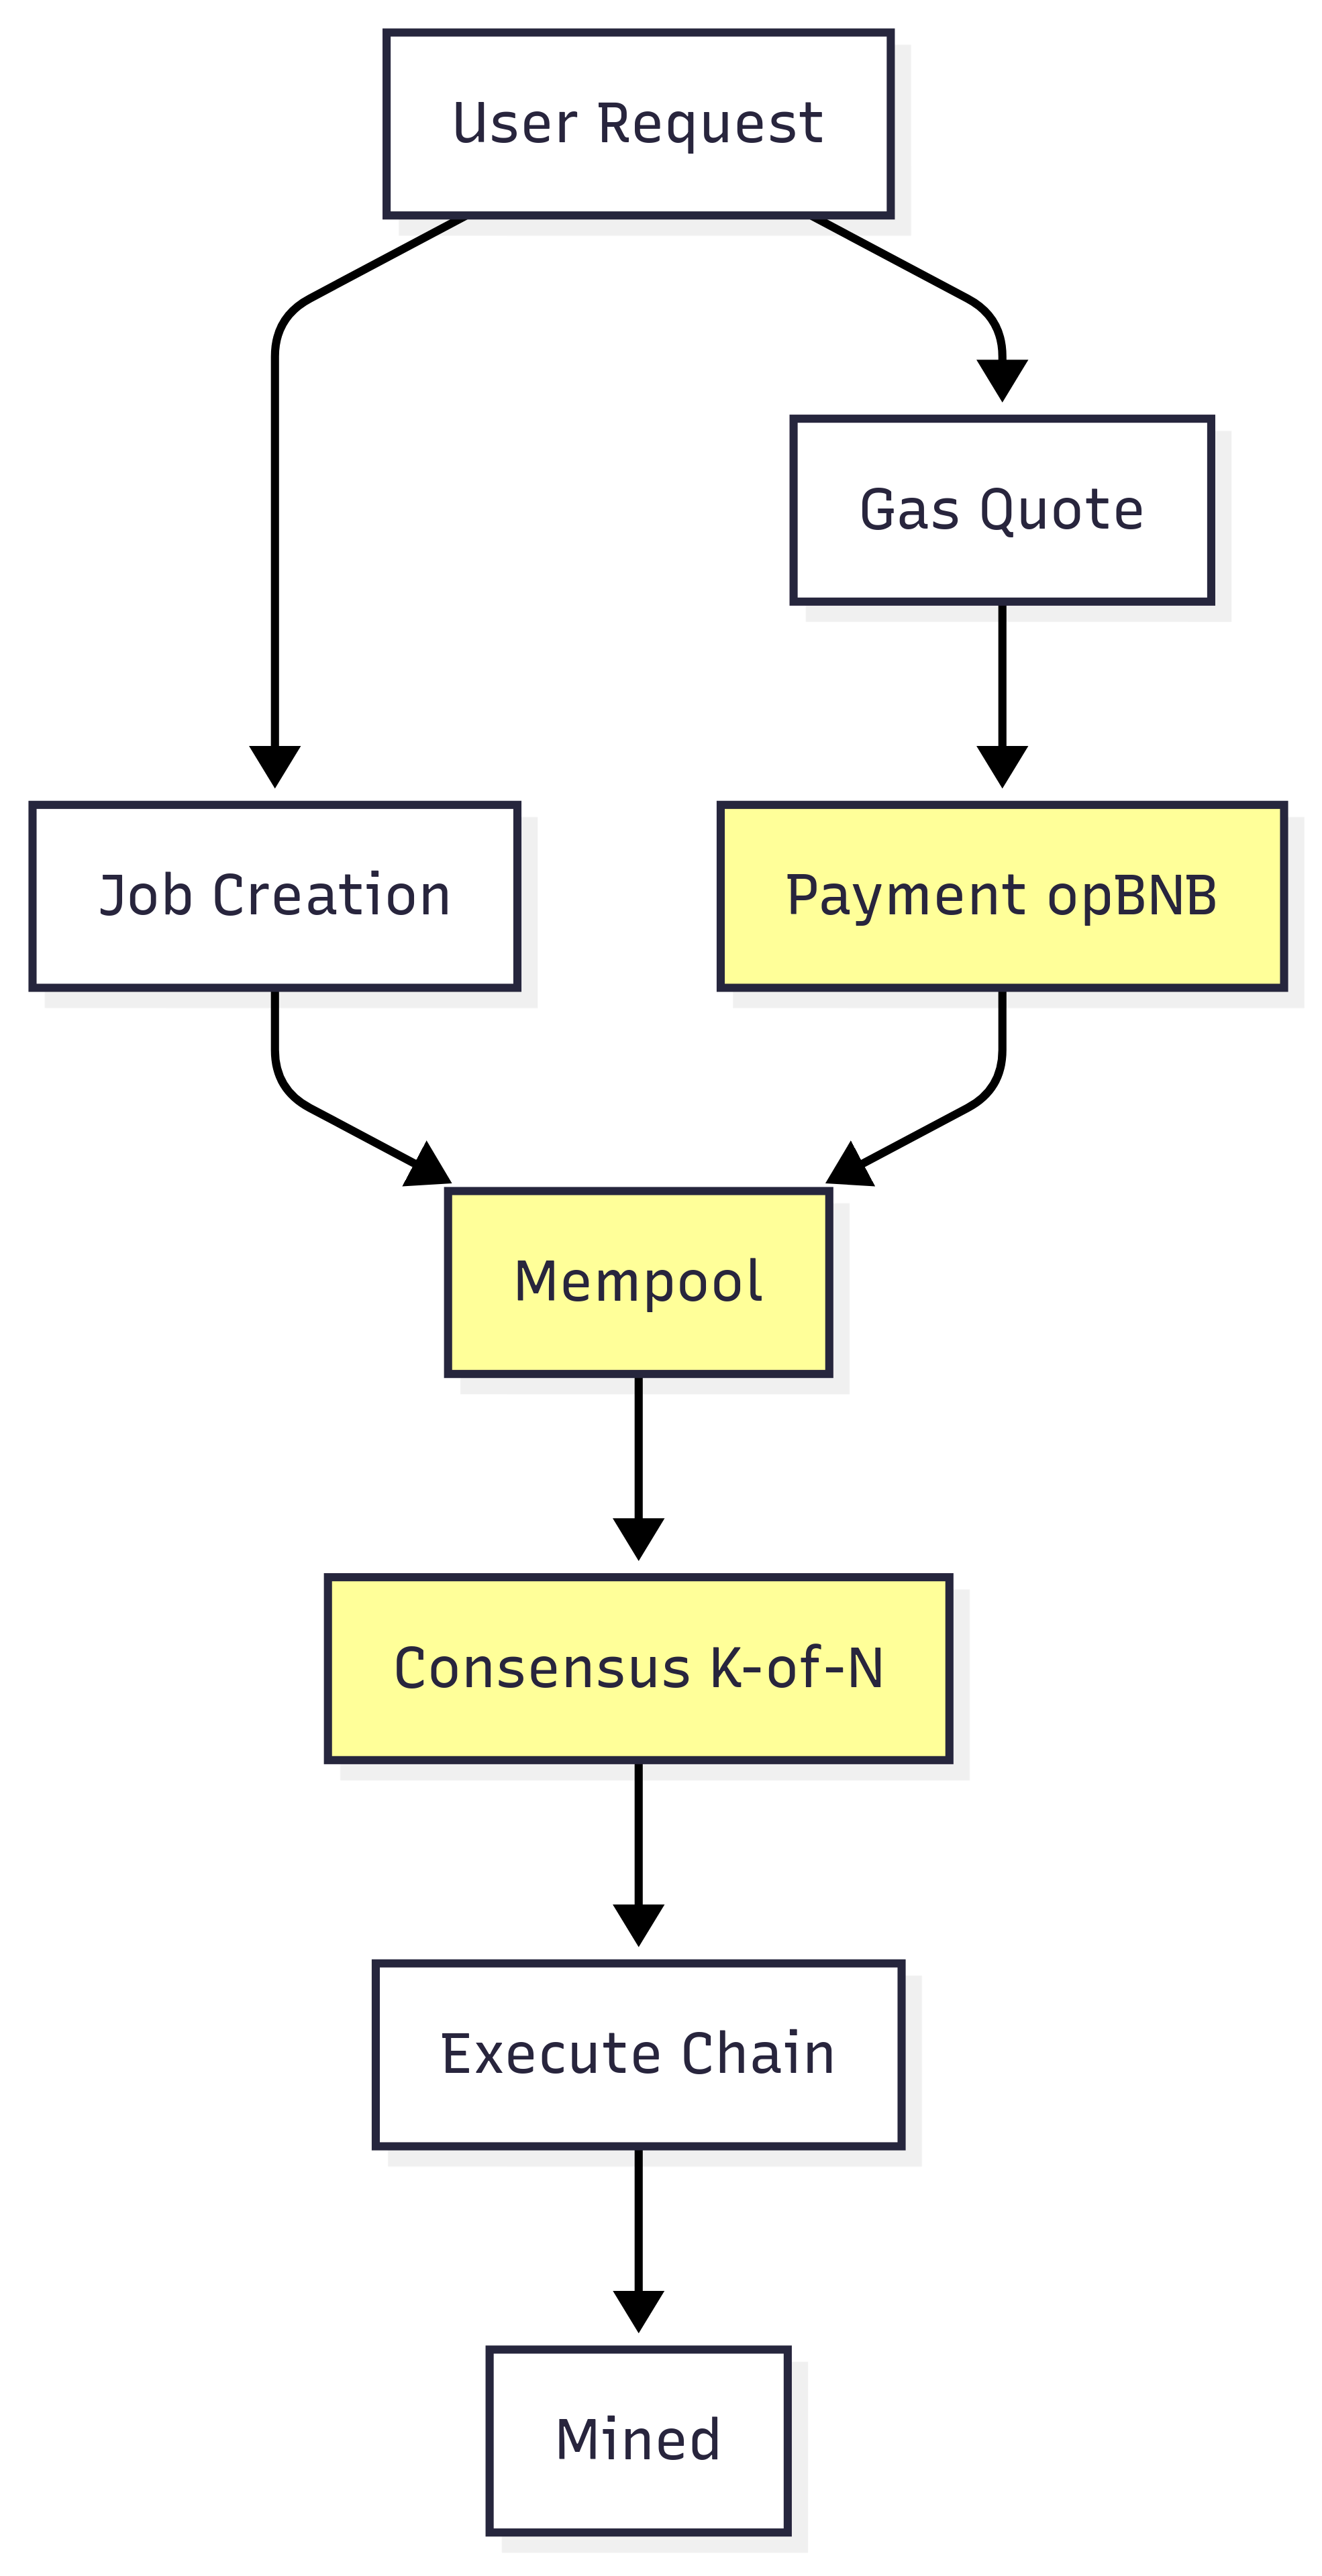
\includegraphics[width=0.5\textwidth]{images/full-flow.png}
  \end{center}

\end{figure}

\subsection{User Request and Job Creation}
The gasless transaction flow begins when a user initiates a cross-chain request by specifying the destination chain and providing the raw transaction details. UGF parses this request and constructs a chain-specific job object, caching it temporarily with a unique digest to prevent replay attacks and to track payment status.

\paragraph{EVM Chains}
For EVM-compatible chains (e.g., Ethereum, BNB Chain), the job includes the following fields, which define the target contract, input data, gas cost quote, and user metadata:

\begin{itemize}
  \item \texttt{from}: the externally owned account (EOA) initiating the request
  \item \texttt{to}: the destination contract address to interact with
  \item \texttt{callData}: ABI-encoded function and parameters
  \item \texttt{chainId}: numeric chain ID of the target chain
  \item \texttt{quoteWei}: estimated gas fee (in wei) for the transaction
  \item \texttt{quoteInBNB}: the equivalent BNB value to be paid on opBNB
  \item \texttt{userNonce}: optional user-supplied nonce (used for replay protection or ordering)
  \item \texttt{validUntil}: expiration timestamp of the quote in milliseconds
  \item \texttt{status}: the current lifecycle status of the job (e.g., \texttt{quoted}, \texttt{paid})
\end{itemize}

These fields are cached in Redis using a unique digest key. Here's a typical example of the stored object:

\begin{lstlisting}[language=JavaScript, caption={EVM Job Object Stored in Redis}]
await redis.hset(`quote:${digest}`, {
  from,
  to,
  callData,
  chainId: chainId.toString(),
  quoteWei: quoteWei.toString(),
  userNonce: userNonce?.toString() ?? "",
  validUntil: validUntil.toString(),
  status: "quoted",
  quoteInBNB: quoteInBNB.toString(),
});
\end{lstlisting}

\paragraph{Solana}
The job captures a base64-encoded serialized Solana transaction\\
(\texttt{transactionInstructionBase64}), which is later deserialized and dry-run to estimate compute units.

\paragraph{Sui}
For Sui, the backend extracts transaction metadata and computes a digest using BLAKE2b hash of the transaction bytes, a random salt, and a timestamp to ensure uniqueness:

\begin{lstlisting}[caption={Sui Job Digest Creation}]
const txKindBytes = base64ToBytes(txKindB64);
const randomSalt = ethers.hexlify(ethers.randomBytes(16));
const timestamp = Date.now().toString();

const combinedData = Buffer.concat([
  txKindBytes,
  Buffer.from(randomSalt.slice(2), "hex"),
  Buffer.from(timestamp, "utf8"),
]);

const digest = "0x" + Buffer.from(
  blake2b(combinedData, { dkLen: 32 })
).toString("hex");
\end{lstlisting}

This digest serves as a unique identifier for the transaction request across chains and is stored temporarily in Redis:

\begin{lstlisting}[language=JavaScript, caption={Caching Job Object in Redis}]
await redis.hset(`quote:${digest}`, {
 suiAddressClient: suiAddressClient,
 txKindB64: txKindB64,
 chainId: chainId.toString(),
 lamports: lamports.toString(),
 quoteInBnbWei: quoteInBnbWei.toString(),
 validUntil: validUntil.toString(),
 status: "quoted",
});

await redis.expire(`quote:${digest}`, QUOTE_TTL_SEC);
\end{lstlisting}

This job object is ephemeral and expires if the user does not confirm and pay within a defined TTL. Once paid, the backend marks it as valid and ready for relayer coordination.

\subsection{Gas Estimation and Quote Delivery}
Once the job object is created, the backend estimates the transaction cost on the destination chain. This process varies per chain type:


\paragraph{EVM Chains}
The backend uses on-chain calls (such as \texttt{eth\_estimateGas}) to simulate the transaction and compute the expected gas usage. This value is then multiplied by the current network gas price to derive the total cost in wei.

\paragraph{Solana}
For Solana, the serialized base64 instruction is deserialized and dry-run via \texttt{simulateTransaction}. The resulting compute unit estimate is mapped to a lamport cost, which is then converted to BNB.

\paragraph{Sui}
The Sui backend uses \texttt{devInspectTransactionBlock} to simulate the transaction. The result includes a breakdown of computation and storage costs, which are combined into a native gas fee estimate.

\paragraph{Quote Conversion}
The estimated native gas cost is then converted into a BNB-equivalent quote using real-time price feeds (e.g., Chainlink, CMC, or backend-signed conversion rates). This BNB quote is returned to the client along with the unique digest and expiry timestamp. The quote is now awaiting user payment on opBNB.

\paragraph{Cost Conversion}
We convert the estimated gas units into BNB and add up to a 10\% slippage:
\[
  \mathrm{Cost}_{\mathrm{BNB}}
    = \mathrm{gasUnits} \times \mathrm{gasPrice}
      \times \frac{\mathrm{BNB}}{\mathrm{nativeToken}}
      \times \bigl(1 + 0.10\bigr)
\]

\subsection{Fuel Payment on opBNB}
To proceed with execution, the user must pay the quoted BNB amount to the UGF FuelStation smart contract deployed on \textbf{opBNB}. This payment acts as a cross-chain gas deposit and is linked to the previously issued digest.

\begin{lstlisting}[language=Solidity, caption={FuelStation Payment Handler}]
function payForFuel(bytes32 digest) external payable {
    require(paid[digest] == 0, "FS : Zero Value");
    paid[digest] = msg.value;
    emit FuelPaid(msg.sender, digest, msg.value);
}
\end{lstlisting}

Upon detecting a valid payment event, the FuelStation emits an on-chain event with the associated \texttt{digest}, amount, and sender address. UGF relayers listen to these events in real time. Once the payment is confirmed and matches the quoted amount, the job is marked as \texttt{ready} in Redis, making it eligible for multi-relayer signing and execution on the destination chain.

This payment mechanism ensures:
\begin{itemize}
  \item \textbf{Replay protection}: Each digest is unique and expires if unpaid.
  \item \textbf{Chain-agnostic flow}: Regardless of the destination chain, payment always occurs on opBNB.
  \item \textbf{Fair metering}: Users only pay after receiving an accurate gas quote.
\end{itemize}

\subsection{Distributed Mempool Validation}

After a successful fuel payment on opBNB, the associated transaction digest is marked as \texttt{ready} in Redis. This state change activates UGF’s distributed validation layer — a decentralized coordination mechanism where multiple relayers independently monitor, verify, and act upon eligible jobs.

The term \textbf{distributed} refers to the architectural design: instead of relying on a single centralized processor, UGF deploys multiple Dockerized relayer instances across different geographic regions or nodes. These stateless containers subscribe to job status events and Redis keyspace changes in real time, enabling scalable and fault-tolerant processing.

Each relayer performs lightweight validation checks:
\begin{itemize}
  \item Confirms that the job is marked \texttt{ready} and has not expired.
  \item Validates that no duplicate submission is in-flight for the same digest.
  \item Prepares the transaction for the final k-of-n consensus signing step.
\end{itemize}

Redis acts as a shared coordination bus and lock manager, ensuring that even in a distributed setup, job contention and double execution are prevented. Relayers compete to acquire short-lived distributed locks per digest before proceeding to the next phase.

This approach ensures high availability, horizontal scalability, and tolerance against relayer downtime — making UGF resilient under heavy load or partial node failures. By containerizing each relayer instance, infrastructure orchestration (e.g., using Kubernetes or Docker Swarm) becomes straightforward, allowing for dynamic autoscaling based on transaction volume.

\subsection{Multisignature Consensus: k-of-n Relayer Signing}

Once a relayer secures a distributed lock on a \texttt{ready} job digest, it enters the consensus signing phase. In UGF v0.5, each job requires exactly two relayer signatures — one from a primary and one from a secondary signer — based on a deterministic hash of the job digest. This ensures balanced distribution without overburdening any single node.

\paragraph{Relayer Assignment via Hashing}

Each digest \( D_i \) is mapped to a unique subset of relayers using modular hashing:

\[
h_i = \texttt{keccak256}(D_i) \bmod n
\]
\[
\text{Primary Relayer: } R_{h_i}, \quad \text{Secondary Relayer: } R_{(h_i + 1) \bmod n}
\]

For example, with \( n = 3 \) relayers and a digest \( D_2 \) such that \( h_2 = 2 \), the assigned signers are:
\[
R_2 \text{ (Primary)}, \quad R_0 \text{ (Secondary)}
\]

This approach guarantees:
\begin{itemize}
  \item Uniform load balancing: Each relayer signs approximately \( \frac{2}{n} \) of total jobs.
  \item Determinism: All relayers can independently compute the responsible signers for any given digest.
\end{itemize}

\paragraph{Load Balance}
On average, each relayer handles
\[
  \mathrm{Workload}_j \approx \frac{2}{n}\times\mathrm{TotalJobs}
\]
jobs.


\paragraph{Signing Flow}

\begin{enumerate}
  \item Each relayer computes the digest hash modulo total relayer count to determine role (primary/secondary/idle).
  \item If assigned, the relayer signs the digest using its private key:
  \[
  \sigma_i = \texttt{Sign}_{sk_i}(D_i)
  \]
  \item Signature is stored in Redis under a namespaced key.
  \item Once both \( \sigma_p \) and \( \sigma_s \) (from primary and secondary) are present, the job status is upgraded to \texttt{approved}.
\end{enumerate}

This model ensures:
\begin{itemize}
  \item \textbf{Minimal trust assumptions:} No single relayer can unilaterally submit a transaction.
  \item \textbf{Scalability:} Relayers operate asynchronously, eliminating bottlenecks.
  \item \textbf{Replay protection:} Redis locks and expiration windows prevent race conditions or duplicate signing.
\end{itemize}

\paragraph{Future Upgrade Path}

While v0.5 uses a fixed 2-of-3 scheme, UGF v0.9 will implement configurable \textbf{k-of-n threshold signing}, where \( k \geq 3 \) out of \( n \) relayers must sign before forwarding:

\[
\exists \, \{ \sigma_1, \sigma_2, ..., \sigma_k \} \subseteq \Sigma, \quad \text{such that} \quad |\Sigma| = n, \quad k \leq n
\]

Benefits of this future design:
\begin{itemize}
  \item \textbf{Byzantine fault tolerance (BFT)} in adversarial conditions.
  \item \textbf{Decentralized control} across larger validator sets.
  \item \textbf{Improved redundancy} across geographic and infrastructure diversity.
\end{itemize}

Consensus logic is enforced off-chain using atomic Redis operations and ephemeral signature caches, maintaining high performance without introducing on-chain latency or cost.

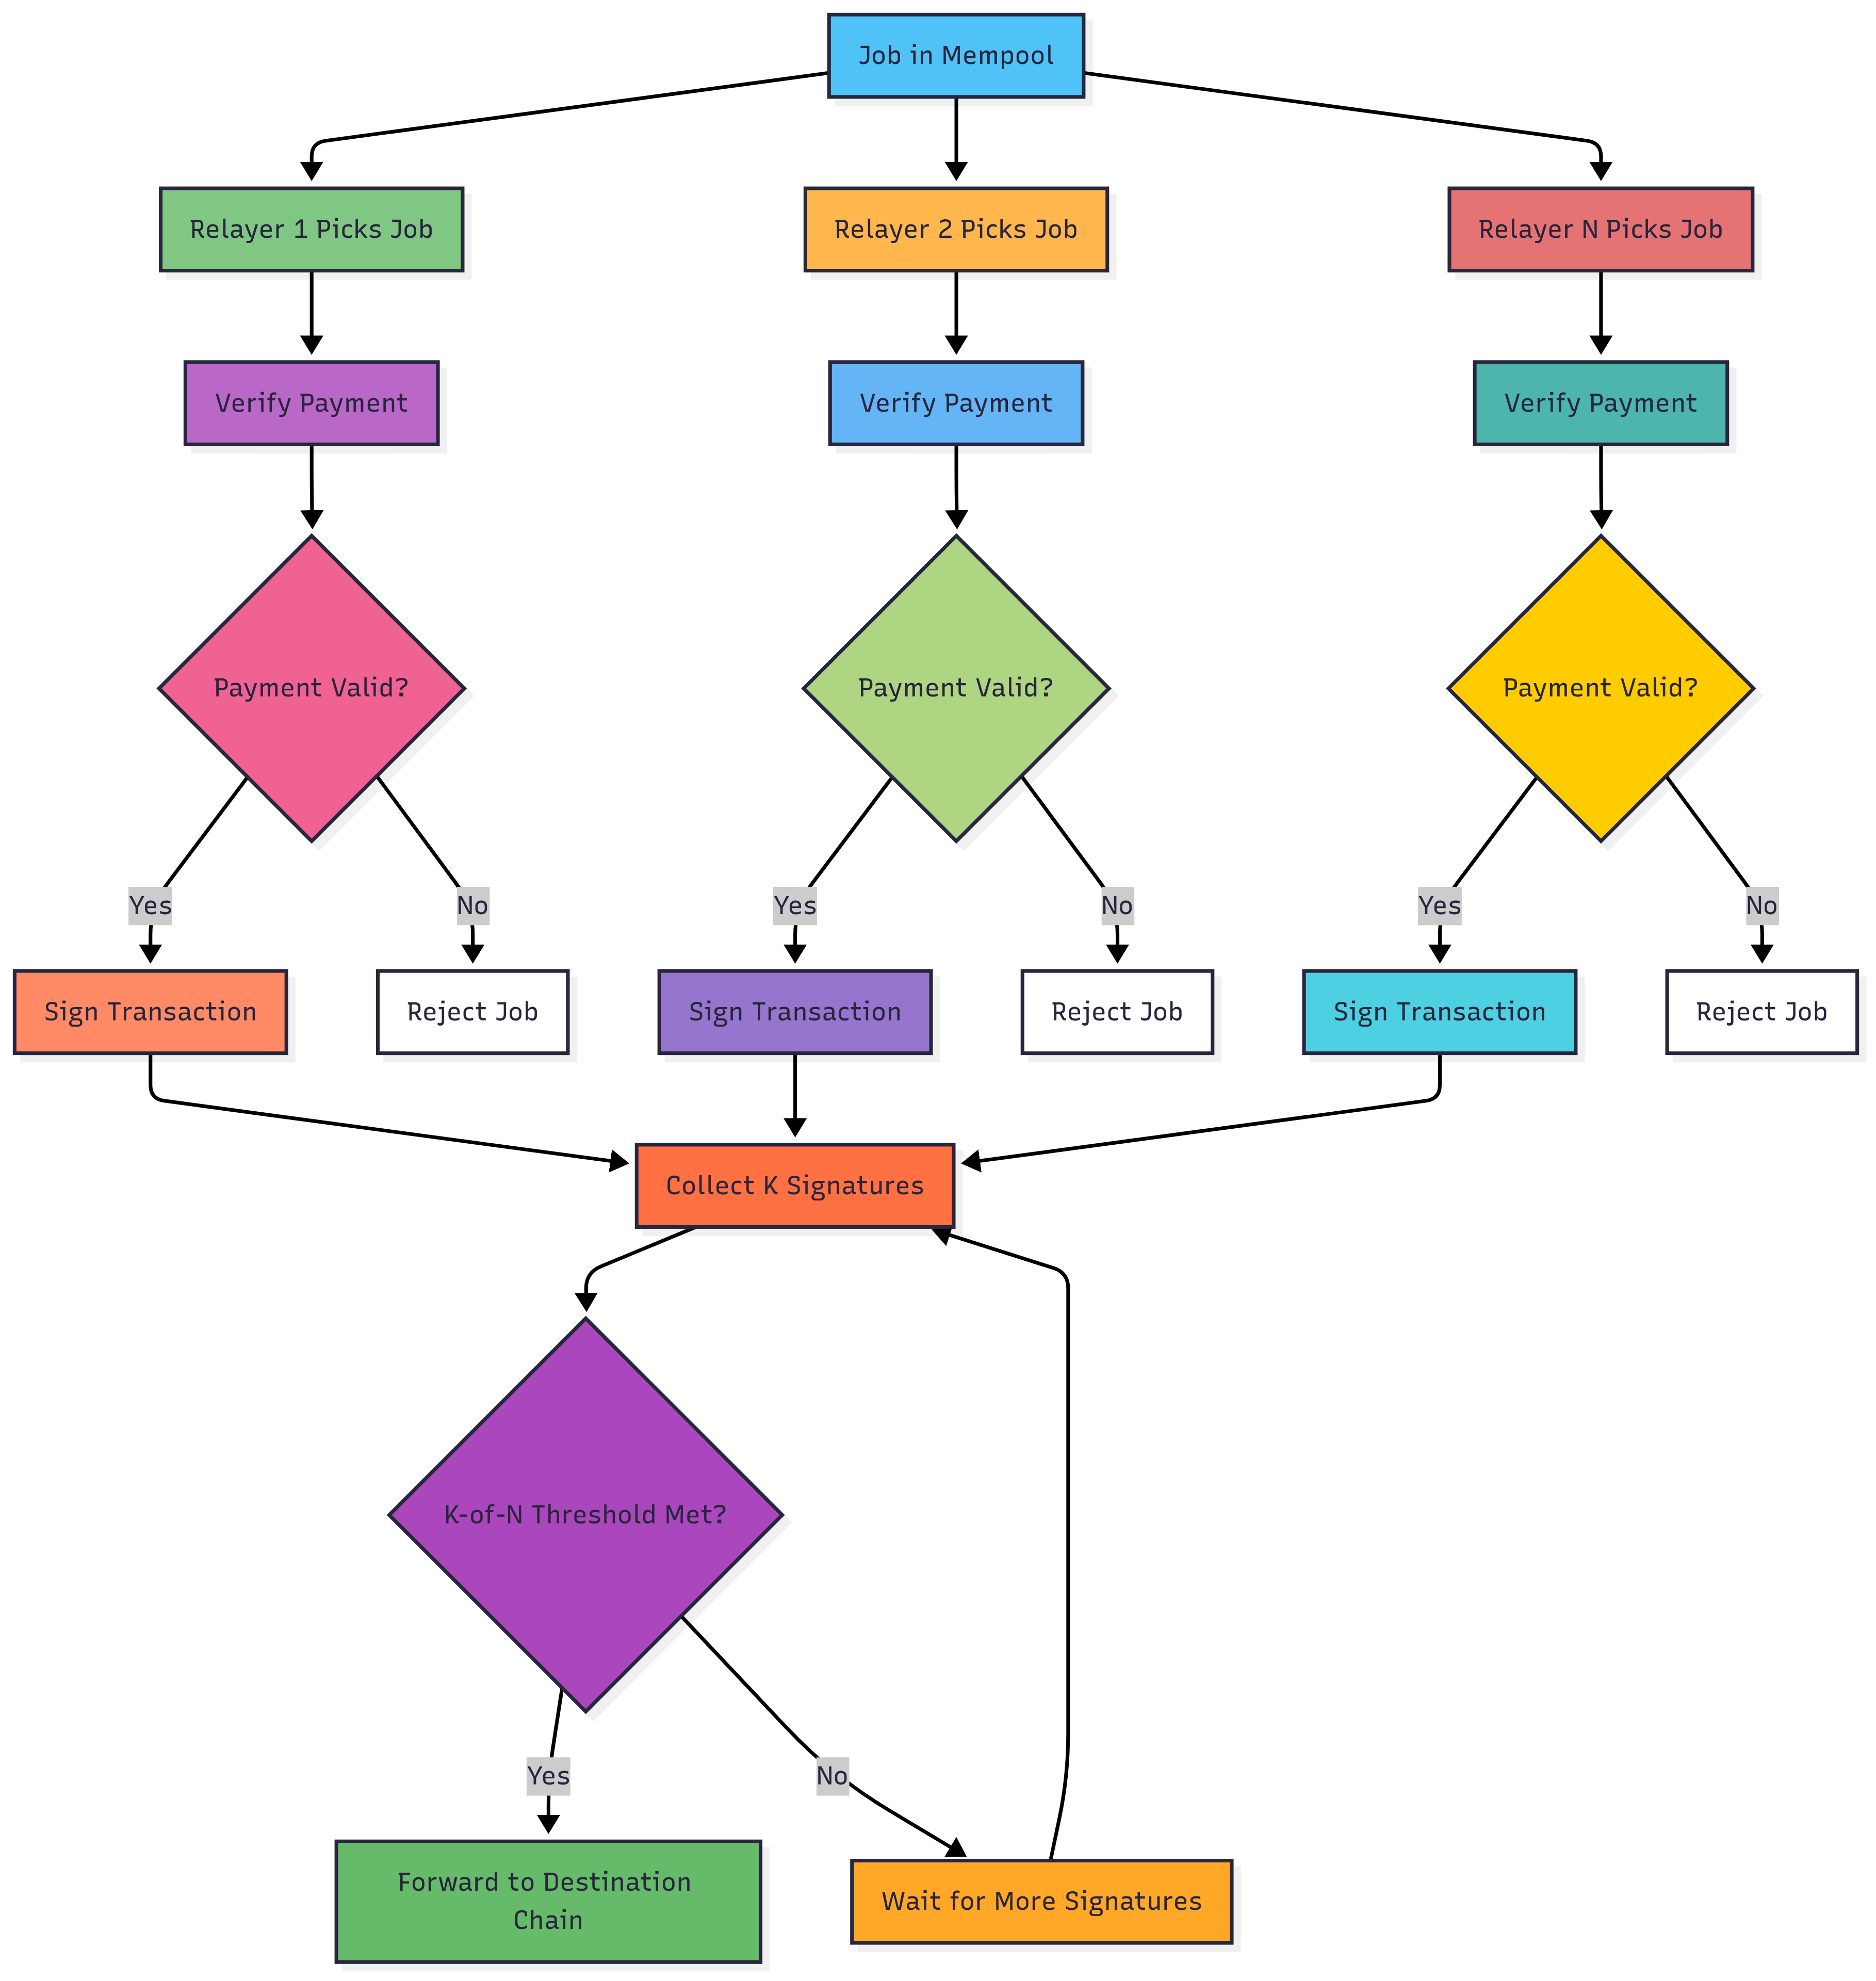
\includegraphics[width=0.9\textwidth]{images/consensus-relayers.png}

\subsection{Destination Chain Execution}

Once a job digest reaches the \texttt{approved} status — meaning it has been signed by the required set of relayers — it is eligible for submission to the destination blockchain.

\paragraph{EVM Chains} 
For EVM-compatible chains, UGF finalizes the transaction by calling the on-chain execution function of a trusted smart wallet or execution contract. This function typically validates the original user's signature and forwards the call to the target contract. An example implementation is shown below:

\begin{lstlisting}[language=Solidity, caption={EVM Smart Execution}]
function executeOp(
    address _to,
    uint256 _value,
    bytes calldata _data,
    bytes calldata _usersignature
) external returns (bytes memory) {
    bytes32 _operationhash = keccak256(
        abi.encodePacked(_to, _value, _data)
    );

    uint256 validationStatus = _validateSignature(
        _operationhash,
        _usersignature
    );
    require(validationStatus == SIG_VALIDATION_SUCCESS,
        "UGF: invalid user operation");

    (bool success, bytes memory returnData) = _to.call{value: _value}(_data);
    require(success, "UGF: execution failed");

    return returnData;
}
\end{lstlisting}

This pattern ensures that only operations properly signed by the original user (and quoted in the UGF flow) are allowed to reach execution. Any tampering with parameters will invalidate the hash and revert the transaction.


\paragraph{Solana} 
UGF reconstructs the original Solana instruction set, signs it with the designated relayer keypair, and submits it via the JSON-RPC `sendTransaction` endpoint. The transaction confirmation is tracked via polling or websockets, and Redis is updated accordingly.

\paragraph{Sui (User-Broadcasted)}
Unlike EVM and Solana, the Sui job is not submitted by UGF. Instead, after receiving UGF’s sponsored gas signature (step shown earlier), the user constructs the full transaction locally and submits it to the Sui network. UGF monitors its completion via the Sui client and marks the job as \texttt{completed} upon success.

\paragraph{Finalization Checks}
Before marking any job as \texttt{completed}, the relayer verifies:
\begin{itemize}
  \item The digest still matches the signed payload.
  \item The transaction receipt (if available) indicates success.
  \item No duplicate submission has occurred.
\end{itemize}

This ensures proper execution across heterogeneous chains with minimal trust and full off-chain coordination.

\subsection{Job Lifecycle Summary}

The complete lifecycle of a gasless cross-chain job in UGF spans seven coordinated phases:

\begin{enumerate}
  \item \textbf{User Request}: The user submits transaction intent (to, calldata, chain, etc.).
  \item \textbf{Gas Estimation \& Quote}: Backend performs dry-run on target chain and issues a BNB quote along with a digest.
  \item \textbf{Fuel Payment}: The user transfers BNB to UGF’s FuelStation on opBNB, tied to the digest.
  \item \textbf{Distributed Validation}: All relayers detect the job status change to \texttt{ready} and verify eligibility.
  \item \textbf{k-of-n Consensus Signing}: Assigned relayers sign the digest and publish their signatures to Redis.
  \item \textbf{Execution}: Upon reaching the signature threshold, a relayer executes the job on the destination chain (or user does for Sui).
  \item \textbf{Finalization}: The backend confirms transaction success, marks the job \texttt{completed}, and emits optional posthooks or events.
\end{enumerate}

This pipeline enables UGF to abstract gas payments, support multi-chain destinations, and maintain a decentralized relayer mesh — ensuring security, reliability, and scale.

\subsection{Security Model and Guarantees}

UGF enforces a multi-step verification process to ensure cross-chain job integrity, payment authenticity, and signer accountability.

\paragraph{1. Digest-Based Uniqueness and Expiry}
Each job is identified by a digest derived from the transaction payload, salt, and timestamp. This prevents reuse and guarantees time-limited validity. Jobs expire if the fuel is not paid within the allowed TTL.

\paragraph{2. Signature Verification}
\begin{itemize}
  \item \textbf{User Signatures} are verified on-chain before transaction execution (EVM) or before gas sponsorship (Sui).
  \item \textbf{Relayer Signatures} follow a defined k-of-n quorum. Only digests with the required number of valid relayer signatures proceed to execution.
\end{itemize}

\paragraph{3. Distributed Relayer Checks}
All relayers independently watch for eligible jobs. Before taking action, each relayer checks:
\begin{itemize}
  \item If the job is marked as ready
  \item If a payment exists for the exact quoted amount
  \item If no one else is already processing the same job
\end{itemize}
This ensures no job is double-processed or skipped.

\paragraph{4. Controlled Fuel Payment}
The on-chain FuelStation contract ensures that:
\begin{itemize}
  \item A digest can only be paid once
  \item The value sent exactly matches the backend quote
\end{itemize}

\paragraph{5. Stateless and Isolated Relayers}
Each relayer runs as a containerized service with no persistent state. If one fails, others continue operating without interruption.

\paragraph{6. Full Job Audit Trail}
Each step — quoting, payment, signing, and execution — is logged with:
\begin{itemize}
  \item User address, chain ID, and digest
  \item Gas quote and payment timestamp
  \item Relayer signature details
  \item Final transaction hash
\end{itemize}

\paragraph{7. Adjustable Signing Threshold}
UGF allows updating the relayer set size \( n \) and required signatures \( k \) before finalization. This helps adapt to network conditions and validator trust levels.

\subsection{Rate Limiting and Abuse Prevention}

While the following mechanisms are currently under internal testing, UGF will enforce strict abuse protection before mainnet launch to ensure reliability and fair usage.

\paragraph{Per-User and IP Limits}
Each user and IP is limited in terms of:
\begin{itemize}
  \item Quote requests per minute
  \item Unpaid job count
  \item Sponsored signature attempts
\end{itemize}
These are tracked via in-memory counters and Redis TTLs.

\paragraph{Quote Expiry}
Unpaid quotes auto-expire after a fixed TTL to prevent stale or abandoned jobs from clogging the system. Each quote auto-expires after TTL:
\[
  \mathrm{expiresAt} = \mathrm{issuedAt} + \mathrm{TTL}
\]

\paragraph{Replay and Spam Filtering}
Duplicate submissions and replayed digests are blocked. Abnormal patterns — like rapid replays or invalid signature bursts — lead to temporary suspensions.

\paragraph{Security Threats and Mitigations}
To ensure the integrity and robustness of the system, UGF employs several security measures against potential attacks. Below is a summary of key threats and their respective mitigations:

\begin{table}[h!]
\centering
\begin{tabular}{|l|l|}
\hline
\textbf{Threat}            & \textbf{Mitigation}                        \\ \hline
Replay attack             & Unique digest + TTL                       \\ \hline
Single-relayer compromise & k-of-n signing threshold                  \\ \hline
Denial-of-service         & Rate limits + IP throttling               \\ \hline
\end{tabular}
\caption{Security Threats and Mitigations}
\end{table}

\paragraph{Future Dynamic Controls}
Before full launch, adaptive throttling will be introduced based on relayer bandwidth, network load, and user reputation.


\subsection{Future Roadmap and Expansion}

After the successful mainnet launch of UGF v1.0, several upgrades are planned to enhance performance, flexibility, and decentralization:

\begin{itemize}
\item \textbf{Security Hardening}: Formal audits, multisig controls, and isolated signer infrastructure to protect keys and minimize attack surfaces.
\item \textbf{DApp SDKs}: Lightweight client SDKs for DApps and wallets to seamlessly integrate UGF gas abstraction into their transaction flows.
\item \textbf{Validator Model (v2.0.0)}: A future version will introduce peer-to-peer validators in a decentralized mesh, removing the need for centralized relayers.
\item \textbf{Own Blockchain Layer}: UGF v2.0 will include its own consensus layer to coordinate validators, validate jobs, and serve as the universal execution rail.
\item \textbf{UGF Scan}: A cross-chain explorer for tracking digests, signatures, and transaction status across all supported networks.
\end{itemize}

\section*{Supported Networks in v1.0.0 (Mainnet)}
\begin{table}[!htb]
\centering
\begin{tabular}{|l|l|}
\hline
\textbf{Network Type} & \textbf{Supported Chains} \\ \hline
Solana & Solana Mainnet (SPL token transfers) \\ \hline
EVM-Compatible & Ethereum, Polygon, Arbitrum, BASE, BNB Smart Chain, Avalanche \\ \hline
Sui & Sui Mainnet \\ \hline
\end{tabular}
\caption{Blockchains supported by UGF in v1.0.0}
\end{table}
\FloatBarrier


\section*{Conclusion}

The \textbf{Universal Gas Framework (UGF)} represents a significant advancement in the evolution of cross-chain interoperability. By leveraging \textbf{BNB on opBNB} as a unified gas currency and integrating a \textbf{distributed relayer consensus} model, UGF seamlessly abstracts away the complexities of managing native gas tokens across multiple blockchains. This not only simplifies the user experience but also facilitates more efficient and secure transactions across disparate blockchain ecosystems.

Through the introduction of \textbf{gasless transactions}, UGF removes the need for users to acquire native tokens on each individual chain, enabling them to focus on their blockchain interactions without worrying about the underlying complexities of gas management. UGF's architecture, built on scalability, security, and modularity, lays the foundation for future cross-chain innovation, making it a cornerstone in the development of decentralized applications (dApps) and blockchain services.

Looking ahead, the \textbf{UGF v1.0} roadmap includes support for additional chains, developer SDKs for easy integration, and the potential for transitioning to a \textbf{validator-driven consensus model}, ensuring the protocol’s robustness and decentralization at scale. As the ecosystem matures, \textbf{UGF} aims to redefine the landscape of cross-chain transaction management, setting a new standard for \textbf{frictionless, gas-abstracted interactions}.

We invite developers, blockchain projects, and early adopters to engage with the \textbf{Tychi Protocol}, contribute feedback, and explore its potential to revolutionize cross-chain interoperability. The future of a unified blockchain ecosystem is within reach, and \textbf{UGF} is at the forefront of this transformation.

\section*{}
\begin{thebibliography}{9}

\bibitem{ethereum}
Ethereum Foundation, \textit{Ethereum Whitepaper}, 2013, \url{https://ethereum.org/en/whitepaper/}

\bibitem{solana}
Solana Labs, \textit{Solana: A New Architecture for a High-Performance Blockchain}, 2020, \url{https://solana.com/}

\bibitem{opbnb}
BNB Chain, \textit{opBNB: Optimism-based Layer 2 Solution}, 2021, \url{https://opbnb.bnbchain.org/}

\bibitem{sui}
Sui Foundation, \textit{Sui: A New Blockchain for Web3}, 2021, \url{https://sui.io/}

\bibitem{suiClient}
Mysten Labs, \textit{SuiClient API Documentation}, 2021, \url{https://sdk.mystenlabs.com/typedoc/classes/_mysten_sui.client.SuiClient.html}

\bibitem{solanaspl}
Solana Labs, \textit{SPL Token Program}, 2020, \url{https://docs.solana.com/developing/programming-model/overview#spl-token-program}

\bibitem{ethgasestimation}
Ethereum Foundation, \textit{Ethereum Gas Estimation}, 2015, \url{https://ethereum.org/en/developers/docs/apis/json-rpc#eth_estimategas}

\bibitem{solanagasestimation}
Solana Labs, \textit{Solana Gas Estimation and Fees}, 2021, \url{https://docs.solana.com/developing/programming-model/fees}

\bibitem{redis}
Redis, \textit{Redis: An open-source, in-memory data structure store}, 2021, \url{https://redis.io/}

\bibitem{tendermint}
Tendermint, \textit{Tendermint: Consensus without Mining}, 2018, \url{https://tendermint.com/static/docs/tendermint.pdf}

\bibitem{typescript}
Microsoft, \textit{TypeScript: A typed superset of JavaScript}, 2021, \url{https://www.typescriptlang.org/}

\end{thebibliography}

\end{document}
